\documentclass[fleqn]{article}
\usepackage{mathtools}
\usepackage{graphicx}
\usepackage{amssymb}
\usepackage[margin = 0.75in]{geometry}
\usepackage{enumerate}
\usepackage{color}
\usepackage{fancyvrb}
\usepackage{breqn}
\usepackage{fancyhdr}
\usepackage{multicol}
%\usepackage[latin1]{inputenc}
\usepackage{tikz}
\usepackage{circuitikz}
\usepackage{pgfplots}
\pgfplotsset{compat=1.8}

\pgfplotsset{vasymptote/.style={
    before end axis/.append code={
        \draw[densely dashed] ({rel axis cs:0,0} -| {axis cs:#1,0})
        -- ({rel axis cs:0,1} -| {axis cs:#1,0});
    }
}}

\renewcommand{\thispagestyle}[1]{}
\pagestyle{fancy}
\lhead{\textbf{NAME:}}
\rhead{}

\begin{document}
\title{Math 120R.002 Exam 3 Version B}
\date{11.13.14}
\maketitle

\section*{Instructions:} 
Please show all of your work for each question. Providing just the final answer \textbf{will not merit full credit}. The best way to ensure full credit is to provide the equation you use, show some work, and mark your final answer in an obvious way (circle, box, underline, etc.). The point values for each question are located at the beginning of the question.

\vspace{1in} 

\begin{tabular}{|p{6.5in}|} 
\hline 
\noindent By signing my name below, I agree that I am following all rules and regulations set forth by the Code of Academic Integrity.  Furthermore, I agree that I am following all rules set by my instructor and by the course policy for this exam.  This includes ensuring that all calculator programs except possibly QUADRATIC FORMULA have been deleted.\\
\vspace{.3 in}\\
\underline{Signature:	\hspace{2.5 in}	Date:\hspace{1.25 in}}\\
\hline 
\end{tabular} 

\vspace{1 in}

Formulas:
\begin{align*}
P(t) & = P_0 e^{rt} & P(t) & = P_0 2^{t/h} & m(t) & = m_0 e^{-rt} & m(t) & = m_0 (\frac{1}{2})^{t/h} & T(t) &= T_s + D_0 e^{-kt} \\
A(t) & = P ( 1 + \frac{r}{n})^{nt} & A(t) & = P e^{rt} & P(t) & = \frac{C}{1 + ke^{-rt}}
\end{align*}

\pagebreak
\thispagestyle{fancy}{
\lhead{}
\rhead{/25}}

\section*{Free Response}

\begin{enumerate}

\item \textit{(5 points)} Solve the following equation for $x$.  You may check your answer with your calculator but you must justify how you got your answer algebraically (by showing your work).
\begin{gather*}
\ln(x-10) - \ln(x+6) = \ln(x-1)
\end{gather*}

\vspace{1.5in}

\item \textit{(20 points)} A car engine runs at a temperature of 200$^\circ$F and then the car is turned off. The engine cools according to Newton's law of cooling.
where $t$ is measured in minutes.
It is 80$^\circ$F outside and the engine reaches a temperature of 126$^\circ$F after half an hour.
\begin{enumerate}
\item What is the cooling constant (k) for the engine, rounded to 5 decimal places?

\vspace{1in}
ANS: \underline{\hspace{2in}}

\item How long will it take for the engine to reach a temperature of 100$^\circ$? (If you do not have an answer for the last part, use 0.0500 as your cooling constant.)

\vspace{1in}
ANS: \underline{\hspace{2in}}


\end{enumerate}

\item \textit{(10 points)} The displacement of a buoy from the surface of the water can be modeled by $d(t) = A\sin(Bt)$.  The maximum displacement from the surface of the water is 2.5 feet.  The time it takes for the buoy to go from zero displacement to its maximum displacement is 5 seconds.  Determine $A$ and $B$ from the given information.

\pagebreak
\thispagestyle{fancy}{
\lhead{}
\rhead{/35}}

\item \textit{(15 points)} A cork floating in a lake is bobbing in simple harmonic motion.
Its displacement $h$ above the bottom of the lake is modeled by
\begin{align*}
h(t) = 3 \cos(10\pi t + 20\pi) + 3
\end{align*}
\begin{enumerate}
\item Find the amplitude, period, average, and phase shift of the motion.

\vspace{1.25in}
Amplitude: \underline{\hspace{.7in}} \qquad Period: \underline{\hspace{.7in}} \qquad Average: \underline{\hspace{.7in}} \qquad Phase Shift: \underline{\hspace{.7in}}

\item Use the axes provided to sketch \textbf{1 full period} of the wave starting at $t = 0$.
Make sure to label the amplitude, period, and average on the graph \\
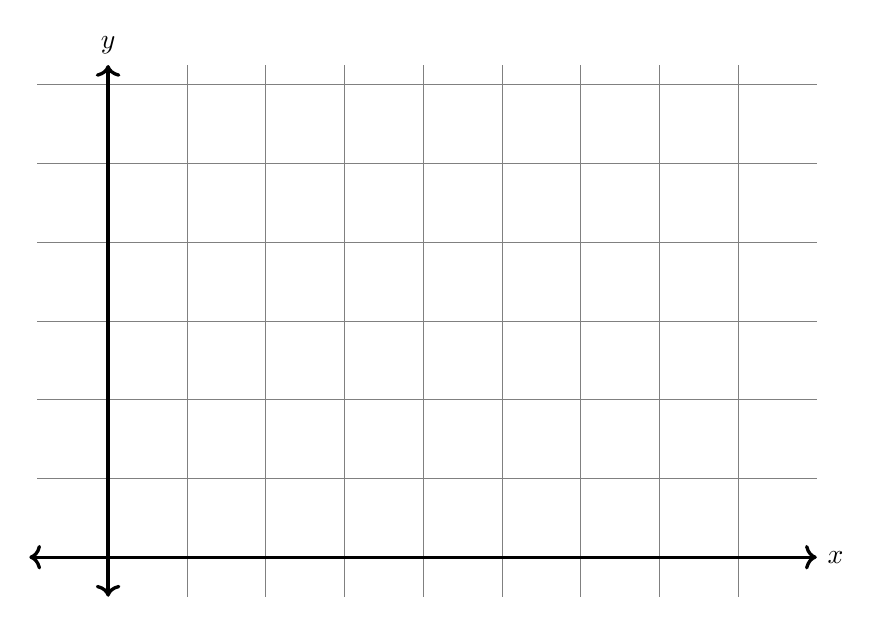
\begin{tikzpicture}[y=1cm, x=10cm]
	\draw[very thin,color=gray, xstep=0.1, ystep=1] (-0.09,-0.5) grid (0.9,6.25);
	\draw[<->, very thick] (-0.1,0) -- (0.9,0) node[right] {$x$};
	\draw[<->, very thick] (0,-0.5) -- (0,6.25) node[above] {$y$};
\end{tikzpicture}

\end{enumerate}

\item \textit{(10 points)} A certain sparrow species was introduced into an area 10 years ago.  Now the population is at 10,000.  Given the following logistic model, answer the following questions.  $t$ are the years since 2005 (i.e. ten years ago).

\begin{align*}
P(t) = \frac{40000}{1+9e^{kt}}
\end{align*}

\begin{enumerate}
\item What is the value for $k$?
\vspace{1.25in}

\item What was the initial population? What is the max population of sparrows that this area can sustain?

\vspace{1in}

Initial Population: \underline{\hspace{1.5in}} \qquad Max Population: \underline{\hspace{1.5in}}

\end{enumerate}

\pagebreak
\thispagestyle{fancy}{
\lhead{}
\rhead{/30}}

\section*{Multiple Choice}

\item (5 points) Suppose a pack of lemurs are experiencing exponential growth.  It is also known they had a population of 4,000 in 1990 and they now have a population of 5,000.  How many lemurs will there be 5 years from now (Rounded down to whole number)?
\begin{multicols}{3}
\begin{enumerate}
\item 4,000
\item 4,182
\item 5,000
\item 5,228
\item 6,000
\item 6,535
\end{enumerate}
\end{multicols}

\vspace{0.3in}

\item \textit{(5 points)} The half-life of cesium-137 is 30 years.  What is the relative (or continuous) rate of decay?  Assume $r$ comes from $m(t) = m_0 e^{-rt}$
\begin{enumerate}
\item 30
\item $\frac{\ln(2)}{30}$
\item $\frac{1}{30}$
\item $\frac{30}{\ln(2)}$
\item $-\frac{30}{\ln(2)}$
\end{enumerate}

\vspace{0.3in}

\item \textit{(5 points)} Consider the following statements, and decide which are true.
\begin{multicols}{2}
\begin{enumerate}[I.]
\item $\sin(x) = \cos(x - \pi/2)$
\item $\cos(x) = -\cos(x + \pi)$
\end{enumerate}
\end{multicols}
\begin{multicols}{3}
\begin{enumerate}
\item Both are true
\item Only I is true
\item Only II is true
\item Neither are true
\end{enumerate}
\end{multicols}

\vspace{0.3in}

\item \textit{(5 points)} Evaluate $\displaystyle \sin^{-1}\left(\sin\left( \frac{11\pi}{6} \right) \right)$.
\begin{multicols}{3}
\begin{enumerate}
\item $\displaystyle \frac{11\pi}{6}$
\item $\displaystyle \frac{-\pi}{6}$
\item $\displaystyle \frac{\pi}{6}$
\item $\displaystyle \frac{-11\pi}{6}$
\item $\displaystyle \frac{-1}{2}$
\end{enumerate} 
\end{multicols}

\vspace{0.3in}

\item \textit{(5 points)} Completely expand the following.
\begin{align*}
\log_3 \left( \frac{A^3 \sqrt{B}}{3CD^2} \right)
\end{align*}
\begin{enumerate}
\item $\log_3(A^3\sqrt{B}) - \log_3(3CD^2)$
\item $3\log_3(A) + \frac{1}{2}\log_3(B) - 1 + \log_3(C) + 2\log_3(D)$
\item $3\log_3(A) + \frac{1}{2}\log_3(B) - 1 - \log_3(C) - 2\log_3(D)$
\item $-3\log_3(A) - \frac{1}{2}\log_3(B) + 1 + \log_3(C) + 2\log_3(D)$
\item none of the above
\end{enumerate}

\vspace{0.3in}

\pagebreak
\thispagestyle{fancy}{
\lhead{}
\rhead{/10}
\rfoot{/100}}

\item (5 points) We know $t$ has a terminal point of $(\frac{3}{5},\frac{4}{5})$.  What is the terminal point for $\pi - t$?

\begin{multicols}{4}
\begin{enumerate}
\item $(\frac{3}{5},\frac{4}{5})$
\item $(-\frac{3}{5},\frac{4}{5})$
\item $(\frac{3}{5},-\frac{4}{5})$
\item $(-\frac{3}{5},-\frac{4}{5})$
\item $(\frac{4}{5},\frac{3}{5})$
\item $(-\frac{4}{5},-\frac{3}{5})$
\end{enumerate}
\end{multicols}

\vspace{0.3in}


\item \textit{(5 points)} The domain of $\sin^{-1}(x)$ is
\begin{multicols}{3}
\begin{enumerate}
\item $[-\frac{\pi}{2}, \frac{\pi}{2}]$
\item $[-1, 1]$
\item $(-\frac{\pi}{2}, \frac{\pi}{2})$
\item $(-1, 1)$
\item $(-\infty, \infty)$
\end{enumerate}
\end{multicols}

\vspace{0.3in}

\item \textit{(5 points)} The range of $\cos^{-1}(\sin(x))$ is
\begin{multicols}{3}
\begin{enumerate}
\item $[0, \pi]$
\item $[-1, 1]$
\item $(0, \pi)$
\item $(-1, 1)$
\item $(-\infty, \infty)$
\end{enumerate}
\end{multicols}

\end{enumerate}

\end{document}